\documentclass[../../main.tex]{subfiles}
\begin{document}

In diesem Kapitel sei stets $\K\in\{\R,\C\}$. Ist $a\in\K$, so schreiben wir wieder $a^*$ für die komplex-konjugierte Zahl [$\to$\ref{4.2.7}] (falls $\K=\R$, so gilt natürlich $a^*=a$).
Allgemeiner schreiben wir $A^*$ für die komplex-konjugierte transponierte Matrix $(a_{ij}^*)_{1\le j\le n,1\le i\le m}\in\K^{n\times m}$ einer Matrix
$A=(a_{ij})_{1\le i\le m,1\le j\le n}\in\K^{m\times n}$ (falls $\K=\R$, so gilt natürlich $A^*=A^T$ [$\to$\ref{9.1.21}]). Zum Beispiel gilt
\[\begin{pmatrix}1+2\i&0&1\\0&-\i&2\end{pmatrix}^*=\begin{pmatrix}1-2\i&0\\0&\i\\1&2\end{pmatrix}.\]

\section{Skalarprodukte}
\begin{df}\label{11.1.1}
Sei $V$ ein $\K$-Vektorraum. Ein \emph{Skalarprodukt}\index{Vektorraum@{\bf Vektorraum}!normierter Vektorraum!Skalarprodukt} auf $V$ ist eine Abbildung $V\times V\to\K,\ (v,w)\mapsto\langle v,w\rangle$ derart, dass für alle
$u,v,w\in V$ und $\la\in\K$ gilt:
\begin{eqnarray}
\langle u+v,w\rangle&=&\langle u,w\rangle+\langle v,w\rangle\\
\langle\la v,w\rangle&=&\la^*\langle v,w\rangle\\
\langle u,v+w\rangle&=&\langle u,v\rangle+\langle u,w\rangle\\
\langle v,\la w\rangle&=&\la\langle v,w\rangle\\
\langle v,w\rangle&=&\langle w,v\rangle^*\\
v\ne0&\implies&\langle v,v\rangle>0
\end{eqnarray}
Für $\K=\R$ sagt man, dass die Abbildung \emph{bilinear} [(1)--(4)] (nämlich \emph{linear im ersten} [(1),(2)] und \emph{zweiten Argument} [(3),(4)]),
\emph{symmetrisch} [(5)] und \emph{positiv definit} [(6)] ist. Für  $\K=\C$ sagt man, dass die Abbildung \emph{sesquilinear}\footnote{"`sesqui"' kommt aus dem Lateinischen und bedeutet "`anderthalb"'.} [(1)--(4)] (nämlich \emph{semilinear oder auch antilinear im ersten} [(1),(2)] und \emph{linear im zweiten Argument} [(3),(4)]),
\emph{hermitesch} [(5)] und \emph{positiv definit} [(6)] ist.
\end{df}

\begin{bem}\label{11.1.2}
\begin{enumerate}[\normalfont(a)]
\item Sei $V$ ein $K$-Vektorraum und $V\times V\to\K,\ (v,w)\mapsto\langle v,w\rangle$ eine Abbildung, die \ref{11.1.1}(4),(5) erfüllt.
Dann gilt $\langle v,0\rangle=\langle v,0_\K\cdot0\rangle=0_\K\langle v,0\rangle=0_\K$ und daher $\langle0,v\rangle=\langle v,0\rangle^*=0_\K^*=0_\K$. Beachte auch, dass
nach (5) gilt $\langle v,v\rangle\in\R$ für alle $v\in V$. Es ist dann
\ref{11.1.1}(6) äquivalent dazu, dass für alle $v\in V$ gilt
\begin{equation}\tag{6'}
\langle v,v\rangle\ge0\qquad\text{und}\qquad(\langle v,v\rangle=0\implies v=0).
\end{equation}
\item Manche Autoren fordern in der Definition eines Skalarprodukts auf einem $\C$-Vektor\-raum die Linearität im ersten und die Semilinearität im zweiten Argument.
Dies ist kein Problem: Um zwischen den beiden Literaturen hin und her zu springen, muss man lediglich die beiden Argumente vertauschen.
\end{enumerate}
\end{bem}

\begin{bsp}\label{11.1.3}
\begin{enumerate}[\normalfont(a)]
\item $\K^n\times\K^n\to\K,\ (x,y)\mapsto\langle x,y\rangle$ definiert durch
\[\langle x,y\rangle:=\sum_{i=1}^nx_i^*y_i=x^*y\qquad\text{für }x=\begin{pmatrix}x_1\\\vdots\\x_n\end{pmatrix},y=\begin{pmatrix}y_1\\\vdots\\y_n\end{pmatrix}\in\K^n\]
ist ein Skalarprodukt auf $\K^n$, das \emph{Standardskalarprodukt}\index{Vektorraum@{\bf Vektorraum}!normierter Vektorraum!Standardskalarprodukt} auf $\K^n$, wobei \ref{11.1.1}(6) folgt aus
$\langle x,x\rangle=\sum_{i=1}^n|x_i|^2$ für alle $x\in\K^n$ [$\to$\ref{4.2.8}].
\item $\R^2\times\R^2\to\R,\ (x,y)\mapsto\langle x,y\rangle$ definiert durch
\[\left\langle\begin{pmatrix}x_1\\x_2\end{pmatrix},\begin{pmatrix}y_1\\y_2\end{pmatrix}\right\rangle:=x_1y_1+5x_1y_2+5x_2y_1+26x_2y_2\qquad\text{für }x_1,x_2,y_1,y_2\in\R\]
ist ein Skalarprodukt auf $\R^2$, denn
$x_1^2+10x_1x_2+26x_2^2=(x_1+5x_2)^2+x_2^2>0$ für $(\begin{smallmatrix}x_1\\x_2\end{smallmatrix})\in\R^2\setminus\{0\}$.
\item Es ist $C([0,1],\K):=\{f\mid f\colon[0,1]\to\K\ \text{stetig}\}$ ein Unterraum des $\K$-Vektorraums $\K^{[0,1]}$ [$\to$\ref{7.1.5}] und
\[C([0,1],\K)\times C([0,1],\K)\to\K,\ (f,g)\mapsto\langle f,g\rangle:=\int_0^1f(x)^*g(x)dx\]
ein Skalarprodukt auf $C([0,1],\K)$, denn $\langle f,f\rangle=\int_0^1f(x)^*f(x)dx=\int_0^1|f(x)|^2dx>0$ falls $f\in C([0,1],\K)\setminus\{0\}$.
\end{enumerate}
\end{bsp}

\begin{df}\label{11.1.4}
Sei $V$ ein $\K$-Vektorraum. Eine \emph{Norm}\index{Vektorraum@{\bf Vektorraum}!normierter Vektorraum!Norm} auf $V$ ist eine Abbildung $V\to\R,\ v\mapsto\|v\|$ derart, dass für alle $v,w\in V$ und $\la\in\K$ gilt
\begin{eqnarray*}
\|v+w\|&\le&\|v\|+\|w\|\qquad\text{"`Dreiecksungleichung"'}\\
\|\la v\|&=&|\la|\|v\|\quad\qquad\text{"`absolute Homogenität"'}\\
v\ne0&\implies&\|v\|>0\qquad\text{[beachte auch $\|0\|=\|0_\K0\|=|0_\K|\|0\|=0_\K$]}
\end{eqnarray*}
\end{df}

\begin{df}\label{11.1.5}
Einen ($\K$-)Vektorraum zusammen mit einem Skalarprodukt oder einer Norm auf $V$ nennt man einen \emph{{\rm($\K$-)}Vektorraum mit Skalarprodukt}\index{Vektorraum@{\bf Vektorraum}!normierter Vektorraum} beziehungsweise einen
\emph{normierten {\rm($\K$-)}Vektorraum}.
\end{df}

\begin{bem}\label{11.1.6}
\begin{enumerate}[\normalfont(a)]
\item
Einen $\K$-Vektorraum mit Skalarprodukt nennt man einen \emph{$\K$-Prä\-hilbert\-raum}, im Fall $\K=\R$ auch einen \emph{euklidischen Raum} und im Fall $\K=\C$ auch einen
\emph{unitären Raum}. Altmodische Autoren sprechen jedoch sowohl im reellen als auch im komplexen Fall von einem unitären Raum, während neumodische Autoren in beiden
Fällen von einem euklidischen Raum sprechen.
\item Formal sind Vektorräume mit Skalarprodukt und normierte Räume bei uns $7$-Tupel, da Vektorräume $6$-Tupel sind [$\to$\ref{6.1.1}]. So wie wir in einer abelschen Gruppe die
Addition fast immer mit $+$ notieren [$\to$\ref{2.1.2}(d)], schreiben wir das Skalarprodukt in einem Vektorraum mit Skalarprodukt fast immer mit $\langle.,.\rangle$ und die Norm
in einem normierten Vektorraum fast immer mit $\|.\|$.
\end{enumerate}
\end{bem}

\begin{lem}\label{11.1.7}
Seien $V$ ein Vektorraum mit Skalarprodukt und $v,w\in V$. Dann \[\langle v+w,v+w\rangle=\langle v,v\rangle+2\rp(\langle v,w\rangle)+\langle w,w\rangle.\]
\end{lem}

\begin{proof}
$\langle v+w,v+w\rangle=\langle v,v+w\rangle+\langle w,v+w\rangle=\langle v,v\rangle+\langle v,w\rangle+\langle w,v\rangle+\langle w,w\rangle\\
=\langle v,v\rangle+\langle v,w\rangle+\langle v,w\rangle^*+\langle w,w\rangle=\langle v,v\rangle+2\rp(\langle v,w\rangle)+\langle w,w\rangle$ [$\to$\ref{4.2.8}]
\end{proof}

\begin{sat}[Cauchy-Schwarz-Ungleichung]\label{11.1.8} \emph{[\href{http://de.wikipedia.org/wiki/Augustin_Louis_Cauchy}{Augustin Louis, baron Cauchy} *1789\\
 \dag 1857, \href{http://de.wikipedia.org/wiki/Hermann_Amandus_Schwarz}{Hermann Amandus Schwarz} *1843 \dag1921]}
Seien $V$ ein Vektorraum mit Skalarprodukt und $v,w\in V$. Dann gilt \[|\langle v,w\rangle|^2\le\langle v,v\rangle\langle w,w\rangle\] mit Gleichheit genau dann,
wenn $v$ und $w$ linear abhängig sind.
\end{sat}

\begin{proof}
Bezeichne $\K$ den Grundkörper von $V$ und setze $S:=\{\ze\in\K\mid|\ze|=1\}$. Dann gilt für $x\in\R$ und $\ze\in S$ nach Lemma \ref{11.1.7}
\[0\le\langle v+x\ze w,v+x\ze w\rangle=\langle v,v\rangle+2x\rp(\ze\langle v,w\rangle)+x^2\langle w,w\rangle.\]
Wähle $\ze\in S$ mit $\rp(\ze\langle v,w\rangle)=|\langle v,w\rangle|$ (nehme $\ze:=\frac{\langle v,w\rangle^*}{|\langle v,w\rangle|}\in S$ falls
$\langle v,w\rangle\ne0$). Dann gilt für alle $x\in\R$
\[0\le\langle v+x\ze w,v+x\ze w\rangle=\langle v,v\rangle+2x|\langle v,w\rangle|+x^2\langle w,w\rangle.\]
Ist $\langle w,w\rangle=0$, so gilt also $\langle v,w\rangle=0$ und $w=0$ ist linear abhängig. Sei also $\langle w,w\rangle>0$.
Die Diskriminante $(2|\langle v,w\rangle|)^2-4\langle w,w\rangle\langle v,v\rangle$ ist dann nicht positiv und genau dann null, wenn $v$ ein skalares Vielfaches von $w$ ist.
\end{proof}

\begin{sat}\label{11.1.9}
Sei $V$ ein Vektorraum mit Skalarprodukt. Dann ist \[V\to\R,\ v\mapsto\|v\|:=\sqrt{\langle v,v\rangle}\] eine Norm auf $V$. Jeder Vektorraum mit Skalarprodukt ist
also auf diese Weise ein normierter Raum.
\end{sat}

\begin{proof} Es ist alles klar bis auf die Dreiecksungleichung: Für alle $v,w\in V$ gilt
\begin{eqnarray*}
\|v+w\|^2&=&\langle v+w,v+w\rangle\\
&\overset{\ref{11.1.7}}=&\langle v,v\rangle+2\rp(\langle v,w\rangle)+\langle w,w\rangle\\
&\overset{\ref{4.2.8}}\le&\langle v,v\rangle+2|\langle v,w\rangle|+\langle w,w\rangle\\
&\overset{\ref{11.1.8}}\le&\langle v,v\rangle+2\|v\|\|w\|+\langle w,w\rangle\\
&=&(\|v\|+\|w\|)^2.
\end{eqnarray*}
\end{proof}

\begin{sat}[Polarisationsformel]\label{11.1.10}
Sei $V$ ein $\K$-Vektorraum mit Skalarprodukt. Dann gilt für alle $v,w\in V$:
\begin{align*}
4\langle v,w\rangle&=\|v+w\|^2-\|v-w\|^2\text{ falls $\K=\R$ und}\\
4\langle v,w\rangle&=\|v+w\|^2-\|v-w\|^2-\i\|v+\i w\|^2+\i\|v-\i w\|^2\text{ falls $\K=\C$.}
\end{align*}
\end{sat}

\begin{proof}
Es gilt $\langle v+w,v+w\rangle-\langle v-w,v-w\rangle=2(\langle v,w\rangle+\langle w,v\rangle)$ für alle $v,w\in V$. Im Fall $\K=\R$, folgt hieraus schon die Behauptung.
Im Fall $\K=\C$ folgt hieraus
$-\i(\langle v+\i w,v+\i w\rangle-\langle v-\i w,v-\i w\rangle)=-2\i(\langle v,\i w\rangle+\langle\i w,v\rangle)=2(\langle v,w\rangle-\langle w,v\rangle)$ für alle $v,w\in V$ und man
braucht dies nur zur obigen Gleichung addieren.
\end{proof}

\begin{defprop}\label{11.1.11}
Seien $V$ ein $\R$-Vektorraum mit Skalarprodukt und $v,w\in V\setminus\{0\}$. Dann existiert eine eindeutig bestimmte Zahl  $\al\in\R$ mit $0\le\al\le\pi$ und
\[\cos\al=\frac{\langle v,w\rangle}{\|v\|\|w\|}.\]
Diese Zahl nennt man den \emph{Winkel}\index{Vektorraum@{\bf Vektorraum}!normierter Vektorraum!Winkel} $\measuredangle(v,w)$ zwischen $v$ und $w$.
\end{defprop}

\begin{proof}
Aus der Analysis weiß man, dass $[0,\pi]\to[-1,1],\ \al\mapsto\cos(\al)$ eine Bijektion ist (die Injektivität folgt daraus, dass diese Funktion streng monoton fällt, und die Surjektivität
aus dem Zwischenwertsatz). Aus der Injektivität dieser Funktion folgt die Eindeutigkeit von $\al$. Aus der Surjektivität folgt die Existenz von $\al$, denn nach Cauchy-Schwarz
\ref{11.1.8} gilt
\[-1\le\frac{\langle v,w\rangle}{\|v\|\|w\|}\le1.\]
\end{proof}

\begin{bem}\label{11.1.12}
\begin{enumerate}[\normalfont(a)]
\item Die durch das Standardskalarprodukt auf dem $\R^2$ [$\to$\ref{11.1.3}(a)] induzierte Norm $\R^2\to\R,\ (\begin{smallmatrix}a\\b\end{smallmatrix})\mapsto\sqrt{a^2+b^2}$
[$\to$\ref{11.1.9}]
gibt gerade die anschauliche Länge eines Vektors im $\R^2$ wieder, wie man leicht sieht, indem man in folgender Zeichnung den Flächeninhalt des großen Quadrats auf
zwei verschiedene Weisen berechnet:
\begin{center}
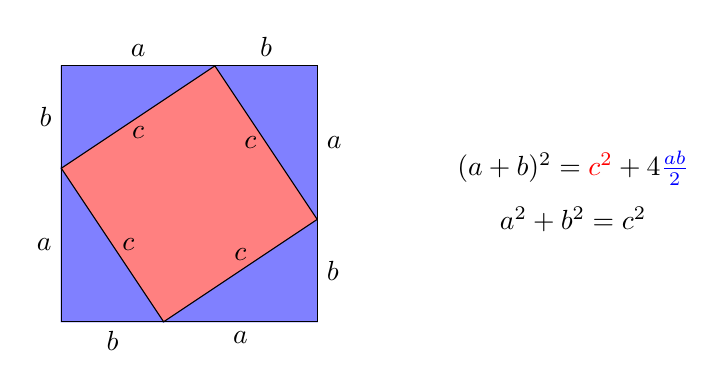
\begin{tikzpicture}[baseline=3em,scale=0.65, execute at begin node=$, execute at end node=$]
\filldraw [color=blue!50](0,0) -- (2,0) -- (0,3) -- cycle;
\filldraw [color=blue!50](0,3) -- (0,5) -- (3,5) -- cycle;
\filldraw [color=blue!50](3,5) -- (5,5) -- (5,2) -- cycle;
\filldraw [color=blue!50](5,2) -- (5,0) -- (2,0) -- cycle;
\draw [fill=red!50] (2,0) -- (3.5,1) node[above]{c} -- (5,2) -- (4,3.5)node[left]{c} -- (3,5) -- (1.5,4)node[below]{c} -- (0,3) -- (1,1.5)node[right]{c} -- cycle;
\draw (0,0) -- (1,0)node[below]{b} -- (3.5,0)node[below]{a} -- (5,0) -- (5,1)node[right]{b} -- (5,3.5)node[right]{a} -- (5,5) -- (4,5)node[above]{b} -- (1.5,5)node[above]{a} -- (0,5) -- (0,4)node[left]{b} -- (0,1.5)node[left]{a} -- (0,0);
\draw (10,3)node {(a+b)^2=\textcolor{red}{c^2}+4\textcolor{blue}{\frac{ab}2}};
\draw (10,2)node {a^2+b^2=c^2};
\end{tikzpicture}
\end{center}
Diesen Sachverhalt bezeichnet man als den Satz von Pythagoras [\href{http://de.wikipedia.org/wiki/Pythagoras}{Pythagoras von Samos} $*\approx$\,-570 \dag~$\approx$\,-510]. Obiges Bild stellt einen "`geometrischen
Beweis"' dar. Es handelt sich um keinen Beweis in unserem Sinne, denn es wird dort anschaulich argumentiert. Es wäre befriedigender, einige Axiome aufzustellen, die noch unstreitbarer  unsere geometrische Anschauung widerspiegeln und den Satz von Pythagoras dann formal aus diesen Axiomen abzuleiten. Letztlich kann man aber ohnehin
nicht vermeiden, gewisse geometrische Tatsachen einfach als gegeben vorauszusetzen (genauer gesagt axiomatisch einzuführen). Man könnte da weiter unten ansetzen, aber das würde viel Zeit kosten und es stellt sich die Frage, warum man es machen sollte. In unserem Rahmen ist daher das obige Bild kein formaler Beweis, aber ein "`Argument"', das den Leser überzeugen soll, dass er sich unter der Norm eines Punktes im $\R^2$ (mit Standardskalarprodukt) den anschaulichen Abstand zum Nullpunkt vorstellen soll.
\item Definition \ref{11.1.11} von Winkeln stimmt überein mit dem anschaulichen Winkelbegriff im $\R^2$ (ausgestattet mit dem Standardskalarprodukt). Wie in (a) argumentieren wir wieder anschaulich: Wegen (a) verändert die Drehung $R_\ph$ ($\ph\in\R$) [$\to$\ref{6.3.2}(a)] die Norm eines Vektors nicht, woraus mit der Polarisationsformel \ref{11.1.10} folgt, dass
$R_\ph$ auch das Skalarprodukt und damit Winkel im Sinne von Definition \ref{11.1.11} nicht verändert. Es reicht also $\measuredangle(v,w)$ für den Fall zu betrachten, dass $v$ auf der Halbachse $\R_{>0}\times\{0\}$ und $w\ne0$
in der oberen Halbebene $\R\times\R_{\ge0}$ liegt (sonst drehe geeignet). Weiter kann man $\|v\|=\|w\|=1$ annehmen, also
$v=(\begin{smallmatrix}1\\0\end{smallmatrix})$ und $w=(\begin{smallmatrix}\cos\be\\\sin\be\end{smallmatrix})$ mit $\be\in[0,\pi]$. Dann gilt für $\al:=\measuredangle(v,w)$,
dass $\cos\al=\langle(\begin{smallmatrix}1\\0\end{smallmatrix}),(\begin{smallmatrix}\cos\be\\\sin\be\end{smallmatrix})\rangle=\cos\be$. Also gilt $\al=\be$, das heißt $\al$ ist der anschauliche Winkel zwischen $v$ und $w$.
\item Die durch das Standardskalarprodukt auf dem $\R^3$ [$\to$\ref{11.1.3}(a)] induzierte Norm $\R^3\to\R,\ \left(\begin{smallmatrix}a\\b\\c\end{smallmatrix}\right)\mapsto\sqrt{a^2+b^2+c^2}$
[$\to$\ref{11.1.9}]
gibt gerade die anschauliche Länge eines Vektors im $\R^2$ wieder, denn nach Pythagoras aus Teil (a) ist die Länge von $\left(\begin{smallmatrix}a\\b\\0\end{smallmatrix}\right)$ gleich $\sqrt{a^2+b^2}$ und wieder nach Pythagoras ist die Länge von $\left(\begin{smallmatrix}a\\b\\c\end{smallmatrix}\right)$ daher $\sqrt{(\sqrt{a^2+b^2})^2+c^2}=
\sqrt{a^2+b^2+c^2}$ (male ein Bild!).
\item Durch Drehung im $\R^3$ sieht man nun wie in (b), dass auch im $\R^3$ der von uns in \ref{11.1.11} eingeführte Winkelbegriff mit dem üblichen übereinstimmt.
\item Sind $a_1,\dots,a_n,b_1,\dots,b_n\in\R$, so gilt im $\C^n$
\begin{align*}
\left\|\begin{pmatrix}a_1+\i b_1\\\vdots\\a_n+\i b_n\end{pmatrix}\right\|&=\sqrt{(a_1-\i b_1)(a_1+\i b_1)+\dots+(a_n-\i b_n)(a_n+\i b_n)}\\
&=\sqrt{a_1^2+b_1^2+\dots+a_n^2+b_n^2}.
\end{align*}
\end{enumerate}
\end{bem}

\section{Orthogonalität}

\begin{df}\label{11.2.1}
Seien $V$ ein $\K$-Vektorraum mit Skalarprodukt und $v,w\in V$. Es heißen $v$ und $w$ \emph{orthogonal} oder \emph{senkrecht zueinander}\index{Vektorraum@{\bf Vektorraum}!normierter Vektorraum!Orthogonalität} (in Zeichen:
$v\perp w$), wenn $\langle v,w\rangle=0$.
\end{df}

\begin{bem}\label{11.2.2}
Seien $V$ ein $\R$-Vektorraum mit Skalarprodukt und $v,w\in V\setminus\{0\}$.
Dann $v\perp w\iff\measuredangle(v,w)=\frac\pi2$ nach der Definition von Winkeln \ref{11.1.11}, denn
$\cos\frac\pi 2=0$. Insbesondere stimmt unsere Definition von Senkrechtstehen in $\R^2$ und $\R^3$ nach \ref{11.1.12} mit unserer geometrischen Anschauung überein. 
\end{bem}

\begin{sat}[Satz von Pythagoras]\label{11.2.3} Sei $V$ ein $\K$-Vektorraum mit Skalarprodukt und seien $v,w\in V$ mit $v\perp w$. Dann $\|v\|^2+\|w\|^2=\|v+w\|^2$ {\rm[$\to$\ref{11.1.9}]}.
\end{sat}

\begin{proof}
$\|v+w\|^2=\langle v+w,v+w\rangle=\langle v,v\rangle+\underbrace{\langle v,w\rangle}_{=0}+\underbrace{\langle w,v\rangle}_{=\langle v,w\rangle^*=0}+\langle w,w\rangle=\|v\|^2+\|w\|^2$.
\end{proof}

\begin{bem}\label{11.2.4} Die Kürze des Beweises des Satzes von Pythagoras in unserem Rahmen, zeigt in eindrucksvoller Weise,
wie einfach man geometrische Sachverhalte mit Hilfe von Skalarprodukten erklären kann. 
Tatsächlich haben wir aber die Gültigkeit des Satzes von Pythagoras schon mehr oder weniger in den Begriff des Skalarprodukts hineinkodiert (und dies in  \ref{11.1.12}
gerechtfertigt). Man könnte daher sagen, dass der \emph{eigentliche} Beweis des Satzes von Pythagoras in \ref{11.1.12}(a) steht. Es stellt aber \ref{11.1.12}(a) nur die Verbindung zur
Anschauung her. Da wir innerhalb unseres Formalismus niemals anschaulich argumentieren, sondern die Anschauung "`nur"' als Inspiration zum Auffinden formaler Beweise
benutzen, wird hier an keiner Stelle gemogelt. 
\end{bem}

\begin{df}\label{11.2.5}\mbox{}[$\to$\ref{6.2.1}]
Sei $V$ ein Vektorraum mit Skalarprodukt. Seien $m\in\N_0$ und $v_1,\dots,v_m\in V$. Dann heißt $(v_1,\dots,v_m)$ ein \emph{Orthonormalsystem (ONS)}\index{Vektorraum@{\bf Vektorraum}!normierter Vektorraum!Orthonormalsystem} (in $V$), wenn
$v_i\perp v_j$ für alle $i,j\in\{1,\dots,m\}$ mit $i\ne j$ und $\|v_i\|=1$ für alle $i\in\{1,\dots,m\}$. Ein ONS, welches $V$ aufspannt, heißt \emph{Orthonormalbasis (ONB)}\index{Vektorraum@{\bf Vektorraum}!normierter Vektorraum!Orthonormalbasis} von $V$.
\end{df}

\begin{bsp}\label{11.2.6}
Die Standardbasis des $\K^n$ [$\to$\ref{6.2.2}] ist eine ONB des $\K^n$ (versehen mit dem Standardskalarprodukt [$\to$\ref{11.1.3}(a)]).
\end{bsp}

\begin{pro}\label{11.2.7}
Sei $V$ ein Vektorraum mit Skalarprodukt und $(v_1,\dots,v_m)$ ein ONS in $V$. Seien $\la_1,\dots,\la_m\in\K$ und $v:=\sum_{i=1}^m\la_iv_i$. Dann
$\la_i=\langle v_i,v\rangle$ für alle $i\in\{1,\dots,m\}$.
\end{pro}

\begin{proof}
$\langle v_j,\sum_{i=1}^m\la_iv_i\rangle=\sum_{i=1}^m\la_i\langle v_j,v_i\rangle=\la_j\
\underbrace{\langle v_j,v_j\rangle}_{=\|v_j\|^2=1}=\la_j$ für alle $j\in\{1,\dots,m\}$
\end{proof}

\begin{kor}\label{11.2.8}
Sei $V$ ein Vektorraum mit Skalarprodukt. In $V$ ist jedes ONS linear unabhängig. Insbesondere ist jede ONB von $V$ eine Basis von $V$.
\end{kor}

\begin{defprop}\label{11.2.9}
Sei $V$ ein Vektorraum mit Skalarprodukt und $U$ ein Unterraum von $V$. Das \emph{orthogonale Komplement}\index{Vektorraum@{\bf Vektorraum}!normierter Vektorraum!orthogonales Komplement} von $U$ in $V$ ist definiert durch
\[U^\perp:=\{v\in V\mid\forall u\in U:v\perp u\}\]
und ist selber wieder ein Unterraum von $V$ mit $U\cap U^\perp=\{0\}$ und $U\subseteq(U^\perp)^\perp$. Ist $U=\lin(E)$ für ein $E\subseteq V$, so gilt
$U^\perp=\{v\in V\mid\forall u\in E:v\perp u\}$.
\end{defprop}

\begin{proof} Sehr einfache Übung.
\end{proof}

\begin{defprop}\label{11.2.10}
Seien $V$ ein Vektorraum mit Skalarprodukt, $U$ ein Unterraum von $V$ und $v\in V$. Dann gibt es höchstens ein $w\in U$ mit $v-w\in U^\perp$. Falls existent, nennt man dieses $w$ die \emph{orthogonale Projektion}\index{Vektorraum@{\bf Vektorraum}!normierter Vektorraum!orthogonale Projektion} von $v$ auf $U$.
\end{defprop}

\begin{proof}
Seien $w,w'\in U$ mit $v-w,v-w'\in U^\perp$. Dann
\[\langle w-w',w-w'\rangle=\langle w-w',(v-w')-(v-w)\rangle=
\langle\underbrace{w-w'}_{\in U},\underbrace{v-w'}_{\in U^\perp}\rangle-\langle\underbrace{w-w'}_{\in U},\underbrace{v-w}_{\in U^\perp}\rangle=0.\]
\end{proof}

\begin{bsp}\label{11.2.11}
\begin{enumerate}[\normalfont(a)]
\item
Sei $V$ ein Vektorraum mit Skalarprodukt und $U$ ein Unterraum von $V$. Ist $v\in U$, so ist $v$ selber die orthogonale Projektion von $v$ auf $U$. Ist
$v\in U^\perp$, so ist sie der Nullvektor.
\item
Betrachte den $\R$-Vektorraum $\R^\N$ der reellen Folgen [$\to$\ref{6.1.5},~\ref{7.1.5}] und darin den Unterraum $V:=\{f\mid f\colon\N\to\R,\exists c\in\R:\forall n\in\N:|f(n)|\le c\}$
der \emph{beschränkten} Folgen sowie den Unterraum $U$ der Folgen mit endlichem Träger [$\to$\ref{6.2.8}(f)]. Dann ist $V$ vermöge
$\langle f,g\rangle:=\sum_{i=1}^\infty\frac1{2^i}f(i)g(i)\ (f,g\in V)$ ein Vektorraum mit Skalarprodukt und $U$ ein Unterraum von $V$. Das orthogonale Komplement
$U^\perp$ von $U$ in $V$ besteht offenbar nur aus der Nullfolge. Ist $f\in V$, so existiert die orthogonale Projektion von $f$ auf $U$ also genau dann, wenn $f\in U$ (und in diesem Fall ist sie $f$).
\end{enumerate}
\end{bsp}

\red{Bis hierher sollten wir am 7. Februar kommen.}

\begin{pro}\label{11.2.12}
Sei $V$ ein Vektorraum mit Skalarprodukt, $(v_1,\dots,v_m)$ ein ONS in $V$, $U:=\lin(v_1,\dots,v_m)$ und $v\in V$. Dann ist
$\sum_{i=1}^m\langle v_i,v\rangle v_i$ die orthogonale Projektion von $v$ auf $U$. Insbesondere existiert diese.
\end{pro}

\begin{proof}
$w:=\sum_{i=1}^m\langle v_i,v\rangle v_i\in U$. Um $v-w\in U^\perp$ zu zeigen, reicht es $\langle v_j,v-w\rangle=0$ für $j\in\{1,\dots,m\}$ zu zeigen. Sei also $j\in\{1,\dots,m\}$.
Dann \[\langle v_j,v-w\rangle=\langle v_j,v-\sum_{i=1}^m\langle v_i,v\rangle v_i\rangle=\langle v_j,v\rangle-\sum_{i=1}^m\langle v_i,v\rangle
\underbrace{\langle v_j,v_i\rangle}_{\in\{0,1\}}=\langle v_j,v\rangle-\langle v_j,v\rangle=0.\]
\end{proof}

\begin{kor}\label{11.2.13}
Sei $V$ ein Vektorraum mit Skalarprodukt und ONB $\underline v=(v_1,\dots,v_n)$. Dann gilt
\[\co_\v(v)=\begin{pmatrix}\langle v_1,v\rangle\\\vdots\\\langle v_n,w\rangle\end{pmatrix}\qquad\text{für jedes }v\in V.\]
\end{kor}

\begin{proof}
Die orthogonale Projektion eines $v\in V$ auf $V$ ist $v$ selber [$\to$\ref{11.2.11}(a)]. Also gilt nach \ref{11.2.12}
$v=\sum_{i=1}^n\langle v_i,v\rangle v_i$ für alle $v\in V$.
\end{proof}

\begin{pro}[Gram-Schmidtsches Orthogonalisierungsverfahren]\label{11.2.14}
Sei $V$ ein Vektorraum mit Skalarprodukt, $(v_1,\dots,v_m)$ ein ONS in $V$, $U:=\lin(v_1,\dots,v_m)$ und $v\not\in U$. Sei dann $w:=\sum_{i=1}^m\langle v_i,v\rangle v_i$
die orthogonale Projektion von $v$ auf $U$ {\rm[$\to$\ref{11.2.12}]}. Dann ist $(v_1,\dots,v_m,\frac{v-w}{\|v-w\|})$ ein ONS und es gilt 
\[\lin(v_1,\dots,v_m,v)=\lin\left(v_1,\dots,v_m,\frac{v-w}{\|v-w\|}\right).\]
\end{pro}

\begin{proof} Sehr einfache Übung.
\end{proof}

\begin{sat}\mbox{}{\rm[$\to$\ref{6.2.18}]}\label{11.2.15} Jeder endlichdimensionale Vektorraum mit Skalarprodukt besitzt eine ONB.
\end{sat}

\begin{proof}
Induktion nach der Dimension, wobei der Induktionsschritt mit Gram-Schmidt \ref{11.2.14} bewerkstelligt wird.
\end{proof}

\begin{kor}\label{11.2.16}
Sei $V$ ein Vektorraum mit Skalarprodukt und $U$ ein endlichdimensionaler Unterraum von $V$. Dann gibt es für jedes $v\in V$ die orthogonale Projektion $P_U(v)$
von $v$ auf $U$ und dadurch wird eine lineare Abbildung $P_U\colon V\to V$ definiert, deren Kern $U^\perp$ und deren Bild $U$ ist. 
\end{kor}

\begin{proof}
Wähle mit \ref{11.2.15} eine ONB $(v_1,\dots,v_m)$ von $U$. Nach \ref{11.2.12} haben wir dann $P_U(v)=\sum_{i=1}^m\langle v_i,v\rangle v_i$ für alle $v\in U$. Mit der Linearität
des Skalarprodukts im zweiten Argument \ref{11.1.1}(3),(4) rechnet man nun sofort die Linearität von $P_U$ nach. Weiter gilt
\begin{multline*}
\ker P_U=\left\{v\in V\mid\sum_{i=1}^m\langle v_i,v\rangle v_i=0\right\}\overset{\ref{11.2.8}}=\{v\in V\mid\langle v_1,v\rangle=\ldots=\langle v_m,v\rangle=0\}\\
\overset{\ref{11.2.9}}=(\lin(v_1,\dots,v_m))^\perp=U^\perp,
\end{multline*}
$U\subseteq\im P_U$ nach \ref{11.2.11}(a) und selbstverständlich $\im P_U\subseteq U$ nach \ref{11.2.10}.
\end{proof}

\begin{pro}\label{11.2.17}
Sei $U$ ein endlichdimensionaler Unterraum des Vektorraums mit Skalarprodukt $V$. Dann gilt $V=U\oplus U^\perp$ {\rm[$\to$\ref{8.2.1}]}. Für endlichdimensionales $V$ gilt
insbesondere $\dim(U)+\dim(U^\perp)=\dim(V)$ {\rm[$\to$\ref{8.2.3}]}.
\end{pro}

\begin{proof}
Für jedes $v\in V$ gilt
\[v=\underbrace{P_U(v)}_{\in U}+\underbrace{(v-P_U(v))}_{\in U^\perp},\]
also $V=U+U^\perp$. Weiter ist die lineare Abbildung
$U\times U^\perp\to U+U^\perp,\ (u,v)\mapsto u+v$ injektiv, denn ist $(u,v)\in U\times U^\perp$ mit $u+v=0$, so folgt
$u=-v\in U\cap U^\perp\overset{\ref{11.2.9}}=\{0\}$.
\end{proof}

\begin{kor}\label{11.2.18}
Sei $U$ ein Unterraum des endlichdimensionalen $\K$-Vektorraums mit Skalarprodukt $V$. Dann $U=(U^\perp)^\perp$.
\end{kor}

\begin{proof}
Nach \ref{11.2.9} gilt $U\subseteq(U^\perp)^\perp$ und mit \ref{11.2.17} angewandt auf $U$ und auf $U^\perp$
haben wir $\dim(U)=\dim(V)-\dim(U^\perp)=\dim((U^\perp)^\perp)$. Benutze nun \ref{6.2.27}.
\end{proof}

\begin{df}\label{11.2.19}
Seien $V$ und $W$ $\K$-Vektorräume mit Skalarprodukt. Dann heißt eine Abbildung $f\colon V\to W$ ein \emph{Homomorphismus von Vektorräumen mit Skalarprodukt}\index{Vektorraum@{\bf Vektorraum}!normierter Vektorraum!Homomorphismus}
(auch \emph{orthogonal} oder \emph{unitär}, ersteres vorwiegend im Fall $\K=\R$ und letzteres vorwiegend im $\K=\C$), wenn $f$ linear ist und für alle $v,w\in V$ gilt
$\langle f(v),f(w)\rangle=\langle v,w\rangle$. Ist sie zusätzlich bijektiv, so heißt sie \emph{Isomorphismus von Vektorräumen mit Skalarprodukt}
[beachte, dass die Injektivität automatisch erfüllt ist, da aus $f(v)=0$ folgt $\langle v,v\rangle=\langle f(v),f(v)\rangle=0$ und daher $v=0$].
\end{df}

\begin{bem}\label{11.2.20}
Aus der Polarisationsformel \ref{11.1.10} folgt, dass man in dieser Definition die Bedingung $\forall v,w\in V:\langle f(v),f(w)\rangle=\langle v,w\rangle$ ersetzen kann durch
\[\forall v\in V:\|f(v)\|=\|v\|.\]
\end{bem}

\begin{bsp}\label{11.2.21}
Wie in \ref{11.1.12}  bereits bemerkt ist $R_\ph\in\End(\R^2)$ für jedes $\ph\in\R$ ein \emph{Automorphismus des $\R^2$ mit Standardskalarprodukt}.
\end{bsp}

\begin{sat}\label{11.2.22}
Seien $V$ und $W$ $\K$-Vektorräume mit Skalarprodukt und sei\\
$\v=(v_1,\dots,v_n)$ eine ONB von $V$. Sei $f\colon V\to W$ linear. Dann ist $f$ genau dann ein
Isomorphismus von Vektorräumen mit Skalarprodukt, wenn $(f(v_1),\dots,f(v_n))$ eine ONB von $W$ ist.
\end{sat}

\begin{proof}
Die eine Richtung ist klar. Für die andere sei $(f(v_1),\dots,f(v_n))$ eine ONB von $W$. Nach \ref{6.3.8} ist $f$ ein Isomorphismus von Vektorräumen.
Seien nun $v,w\in V$, etwa $v=\sum_{i=1}^n\la_iv_i$ und $w=\sum_{i=1}^n\mu_iv_i$ mit $\la_i,\mu_i\in\K$. Zu zeigen ist $\langle f(v),f(w)\rangle=\langle v,w\rangle$. Es gilt
\begin{align*}
\langle f(v),f(w)\rangle&=\left\langle\sum_{i=1}^n\la_if(v_i),\sum_{j=1}^n\mu_jf(v_j)\right\rangle=\sum_{i,j=1}^n\la_i^*\mu_j\langle f(v_i),f(v_j)\rangle\\
&=\sum_{i=1}^n\la_i^*\mu_i=\sum_{i,j=1}^n\la_i^*\mu_j\langle v_i,v_j\rangle=\left\langle\sum_{i=1}^n\la_iv_i,\sum_{j=1}^n\mu_jv_j\right\rangle=\langle v,w\rangle.
\end{align*}
\end{proof}

\begin{kor}\label{11.2.23} Sei $n\in\N_0$. Je zwei $n$-dimensionale $\K$-Vektorräume mit Skalarprodukt sind als solche isomorph.
\end{kor}

\begin{proof}
Seien $V$ und $W$ $n$-dimensionale $\K$-Vektorräume mit Skalarprodukt. Wähle Orthonormalbasen $(v_1,\dots,v_n)$ von $V$ und $(w_1,\dots,w_n)$ von $W$. Dann ist die lineare
Abbildung $f\colon V\to W$ mit $f(v_i)=w_i$ für $i\in\{1,\dots,n\}$ [$\to$\ref{6.3.4}] ein Isomorphismus von Vektorräumen mit Skalarprodukt.
\end{proof}

\begin{kor}\label{11.2.24}
Sei $V$ ein Vektorraum mit Skalarprodukt und $\v=(v_1,\dots,v_n)$ eine Basis von $V$. Dann sind äquivalent:
\begin{enumerate}[\rm(a)]
\item $\v$ ist ONB von $V$,
\item $\ve_\v\colon\K^n\to V$ ist ein Isomorphismus von Vektorräumen mit Skalarprodukt.
\item $\co_\v\colon V\to\K^n$ ist ein Isomorphismus von Vektorräumen mit Skalarprodukt.
\end{enumerate}
\end{kor}

\begin{df}\label{11.2.25}
Eine Matrix $A\in\K^{n\times n}$ heißt \emph{orthogonal}\index{Matrix@{\bf Matrix}!Orthogonalität} (vor allem wenn $\K=\C$ manchmal auch \emph{unitär}), wenn $f_A$ ein Isomorphismus des Vektorraums $\K^n$
mit dem Standardskalarprodukt ist.
\end{df}

\begin{sat}\label{11.2.26}
Seien $V$ und $W$ Vektorräume mit Skalarprodukt und Orthonormalbasen $\v=(v_1,\dots,v_n)$ und $\w=(w_1,\dots,w_n)$. Sei $f\colon V\to W$ linear. Dann gilt:
\[\text{$f$ ist Isomorphismus von Vektorräumen mit Skalarprodukt}\iff\text{$M(f,\v,\w)$ orthogonal}.\]
\end{sat}

\begin{proof}
Nach \ref{7.1.1} gilt $f=\ve_\w\circ f_{M(f,\v,\w)}\circ\co_\v$ und daher $f_{M(f,\v,\w)}=\co_\w\circ f\circ\ve_\v$. Da $\ve_\w$, $\co_\v$, $\co_\w$ und $\ve_\v$ nach \ref{11.2.24}
Isomorphismen von Vektorräumen mit Skalarprodukt sind, ist $f$ ein solcher genau dann, wenn $f_{M(f,\v,\w)}$ einer ist.
\end{proof}

\begin{sat}\label{11.2.27}
Sei $A\in\K^{n\times n}$. Dann sind äquivalent:
\begin{enumerate}[\rm(a)]
\item $A$ ist orthogonal.
\item Die Spalten von $A$ bilden eine ONB des $\K^n$.
\item Die Zeilen von $A$ bilden eine ONB des $\K^n$.
\item $A^*A=I_n$
\item $AA^*=I_n$
\item $A$ ist invertierbar mit $A^{-1}=A^*$.
\end{enumerate}
\end{sat}

\begin{proof}
Aus \ref{11.2.25}, \ref{11.2.6} und \ref{11.2.22} folgt (a)$\iff$(b), da $f_A(e_1),\dots,f_A(e_n)$ die Spalten von $A$ sind. Direkt aus der Definition der Matrizenmultiplikation
\ref{7.2.1} folgen (b)$\iff$(d) und (c)$\iff$(e). Schließlich gilt (d)$\iff$(e)$\iff$(f) wegen \ref{7.2.13}.
\end{proof}

\begin{bsp}\label{11.2.28}\mbox{}{\rm[$\to$\ref{7.1.4}(a)]}
$\begin{pmatrix}\cos\ph&-\sin\ph\\\sin\ph&\cos\ph\end{pmatrix}$ ist für jedes $\ph\in\R$ orthogonal.
\end{bsp}

\section{Diagonalisierung symmetrischer und hermitescher Matrizen}

\begin{df}\label{11.3.1}
Sei $V$ ein Vektorraum mit Skalarprodukt und $f\in\End(V)$. Dann heißt $f$ \emph{selbstadjungiert}\index{Vektorraum@{\bf Vektorraum}!normierter Vektorraum!selbsadjungierter Endomorphismus} {\rm(}auch \emph{symmetrisch} oder \emph{hermitesch}, ersteres vorwiegend im Fall $\K=\R$ und letzteres vorwiegend im $\K=\C${\rm)}, wenn
$$\langle f(v),w\rangle=\langle v,f(w)\rangle\qquad\text{für alle $v,w\in V$}.$$
\end{df}

\begin{bsp}\label{11.3.2} Die orthogonale Projektion $P_U\in\End(V)$ auf einen endlichdimensionalen Unterraum $U$ eines Vektorraums mit Skalarprodukt $V$ [$\to$\ref{11.2.16}] ist selbstadjungiert. In der Tat: Wegen $V=U+U^\perp$ [$\to$\ref{8.2.1}] reicht es zu beobachten, dass für alle $u_1,u_2\in U$ und $v_1,v_2\in U^\perp$ gilt
$\langle P_U(u_1+v_1),u_2+v_2\rangle=\langle u_1,u_2+v_2\rangle=\langle u_1,u_2\rangle$ und
$\langle u_1+v_1,P_U(u_2+v_2)\rangle=\langle u_1+v_1,u_2\rangle=\langle u_1,u_2\rangle$.
\end{bsp}

\begin{df}\label{11.3.3}
Eine Matrix $A\in\K^{n\times n}$ heißt \emph{selbstadjungiert} {\rm(}im Fall $\K=\R$ auch \emph{symmetrisch}\index{Matrix@{\bf Matrix}!selbstadjungiert}, im Fall $\K=\C$ auch \emph{hermitesch}{\rm)}, wenn $f_A\in\End(\K^n)$ selbstadjungiert ist.
\end{df}

\begin{sat}\label{11.3.4}
Sei $V$ ein Vektorraum mit Skalarprodukt und ONB $\v=(v_1,\dots,v_n)$.
Sei $f\in\End(V)$. Dann gilt: $\text{$f$ selbstadjungiert} \iff\text{$M(f,\v)$ selbstadjungiert}$.
\end{sat}

\begin{proof} Es gilt $f=\ve_\v\circ f_{M(f,\v)}\circ\co_\v$ [$\to$\ref{7.1.1}] und daher
$f\circ\ve_\v=\ve_\v\circ f_{M(f,\v)}$. Da $\v$ eine ONB ist, ist $\ve_\v$ nach \ref{11.2.24} ein Isomorphismus
von Vektorräumen mit Skalarprodukt. Es gilt daher
\begin{align*}
&\text{$f$ selbstadjungiert}\\
\iff&\forall v,w\in V\colon\langle f(v),w\rangle=\langle v,f(w)\rangle\\
\iff&\forall x,y\in\K^n\colon\langle f(\ve_\v(x)),\ve_\v(y)\rangle=\langle\ve_\v(x),f(\ve_\v(y))\rangle\\
\iff&\forall x,y\in\K^n\colon\langle \ve_\v(M(f,\v)x),\ve_\v(y)\rangle=\langle\ve_\v(x),\ve_\v(M(f,\v)y)\rangle\\
\iff&\forall x,y\in\K^n\colon\langle M(f,\v)x,y\rangle=\langle x,M(f,\v)y\rangle\\
\iff&\text{$M(f,\v)$ selbstadjungiert}.
\end{align*}
\end{proof}

\begin{pro}\label{11.3.5}
Seien $K$ ein kommutativer Ring, $m,n,r\in\N_0$, $A\in K^{m\times n}$ und $B\in K^{n\times r}$. Dann gilt:
\begin{enumerate}[\rm(a)]
\item $(AB)^T=B^TA^T$
\item $(AB)^*=B^*A^*$ falls $K=\K$
\end{enumerate}
\end{pro}

\begin{proof}
(a) Schreibt man $A=(a_{ij})_{1\le i\le m,1\le j\le n}$, $B=(b_{jk})_{1\le j\le n,1\le k\le r}$, so gilt
\[(AB)^T\overset{\ref{7.2.1}}{\underset{\ref{9.1.21}}=}\left(\sum_{j=1}^na_{ij}b_{jk}\right)_{1\le k\le r,1\le i\le m}=\left(\sum_{j=1}^nb_{jk}a_{ij}\right)_{1\le k\le r,1\le i\le m}\overset{\ref{7.2.1}}{\underset{\ref{9.1.21}}=}B^TA^T.\]
(b) Ist $K=\K$, so gilt
\[(AB)^*\overset{\ref{7.2.1}}{\underset{\ref{9.1.21}}=}\left(\sum_{j=1}^n(a_{ij}b_{jk})^*\right)_{1\le k\le r,1\le i\le m}\overset{\ref{4.2.7}}=\left(\sum_{j=1}^nb_{jk}^*a_{ij}^*\right)_{1\le k\le r,1\le i\le m}\overset{\ref{7.2.1}}{\underset{\ref{9.1.21}}=}B^*A^*.\]
\end{proof}

\begin{lem}\label{11.3.6}
Sei $A\in\K^{n\times n}$ und $x,y\in\K^n$. Dann gilt $\langle A^*x,y\rangle=\langle x,Ay\rangle$.
\end{lem}

\begin{proof}
$\langle A^*x,y\rangle\overset{\ref{11.1.3}(a)}=(A^*x)^*y\overset{\ref{11.3.5}}=x^*(A^*)^*y=x^*Ay\overset{\ref{11.1.3}(a)}=\langle x,Ay\rangle$
\end{proof}

\begin{pro}\label{11.3.7}
Für $A\in\K^{n\times n}$ gilt
$$\text{$A$ selbstadjungiert}\iff A^*=A.$$
\end{pro}

\begin{proof}
\begin{eqnarray*}
\text{$A$ selbstadjungiert}&\overset{\over{\scriptstyle\ref{11.3.3}}{\scriptstyle\ref{11.3.1}}}\iff&\forall x,y\in\K^n\colon\langle Ax,y\rangle=\langle x,Ay\rangle\\
&\overset{\ref{11.3.6}}\iff&\forall x,y\in\K^n\colon\langle Ax,y\rangle=\langle A^*x,y\rangle\\
&\iff&A=A^*
\end{eqnarray*}
\end{proof}

\begin{lem}\label{11.3.8}
Sei $A\in\K^{n\times n}$ selbstadjungiert und $\la\in\C$ mit $\ch_A(\la)=0$. Dann gilt
$\la\in\R$.
\end{lem}

\begin{proof} Wir können $\K=\C$ annehmen. Dann ist $\la$ ein Eigenwert von $A$ [$\to$\ref{10.1.2},\\
\ref{10.1.3}(e)], das heißt es gibt
$x\in\C^n\setminus\{0\}$ mit $Ax=\la x$. Es folgt
$$\la\langle x,x\rangle\overset{\ref{11.1.1}(4)}=\langle x,\la x\rangle=\langle x,Ax\rangle\underset{\ref{11.3.1}}{\overset{\ref{11.3.3}}=}\langle Ax,x\rangle=\langle\la x,x\rangle
\overset{\ref{11.1.1}(2)}=\la^*\langle x,x\rangle$$
und daher $\la=\la^*$ nach \ref{11.1.1}(6).
\end{proof}

\begin{sat}\footnote{Im Beweis dieses Satzes benutzen wir den Fundamentalsatz der Algebra \ref{4.2.12} [$\to$\ref{4.2.13}(g)].} \label{11.3.9} Sei $V$ ein endlichdimensionaler
Vektorraum mit Skalarprodukt und $f$ ein selbstadjungierter Endomorphismus von $V$. Dann gibt es eine ONB von $V$, die aus Eigenvektoren von $f$ zu reellen Eigenwerten besteht.
Insbesondere ist $f$ diagonalisierbar {\rm[$\to$\ref{10.3.3}(b)]}.
\end{sat}

\begin{proof} Induktion nach $n:=\dim V$.

\noindent
\underline{$n=0$}\quad nichts zu zeigen

\noindent
\underline{$n-1\to n\ (n\in \N)$}\quad Wir zeigen zunächst mit Hilfe von \ref{10.1.7}, dass $f$ einen \emph{reellen} Eigenwert $\la$
besitzt: Wählt man nämlich eine ONB $\w$ von $V$ [$\to$\ref{11.2.15}] und setzt $A:=M(f,\w)$, so ist $A$
nach \ref{11.3.4} selbstadjungiert und daher jedes $\la\in\C$ mit $\ch_A(\la)=0$ nach Lemma \ref{11.3.8} sogar aus $\R$. Nun gilt aber $\ch_f=\ch_A$ [$\to$\ref{10.1.5},~\ref{10.1.9}(e)]
und es gibt ein solches $\la$ wegen $\deg\ch_f\overset{\ref{10.1.6}}=n\ge 1$ nach dem Fundamentalsatz der Algebra \ref{4.2.12}.

Wir wählen nun einen Eigenvektor $u\in V$ zu diesem Eigenwert $\la\in\R$. Setze $U:=\lin(u)$. Da
$f$ selbstadjungiert ist, gilt $f(U^\perp)\subseteq U^\perp$, denn ist $v\in U^\perp$, so gilt
$\langle f(v),u\rangle=\langle v,f(u)\rangle=\la\langle v,u\rangle=0$. Nun ist $f|_{U^\perp}\colon U^\perp\to U^\perp,
v\mapsto f(v)$ ein selbstadjungierter Endomorphismus des Vektorraums mit Skalarprodukt $U^\perp$.
Es gilt $1+\dim(U^\perp)=\dim(U)+\dim(U^\perp)\overset{\ref{11.2.17}}=\dim(V)=n$,
also $\dim(U^\perp)=n-1$. Nach Induktionsvoraussetzung gibt es eine ONB
$(v_2,\dots,v_n)$ von $U^\perp$, die aus Eigenvektoren von $f$ zu reellen Eigenwerten besteht.
Setzt man $v_1:=\frac u{\|u\|}$, so erhält man eine ONB $(v_1,\dots,v_n)$ von
$V$, die aus Eigenvektoren von $f$ zu reellen Eigenwerten besteht.
\end{proof}

\begin{kor}\footnote{Im Beweis dieses Korollars benutzen wir den Fundamentalsatz der Algebra \ref{4.2.12} [$\to$\ref{4.2.13}(g)].}\label{11.3.10}
Sei $A\in\K^{n\times n}$ selbstadjungiert. Dann gibt es eine
\emph{reelle} Diagonalmatrix $D\in\R^{n\times n}$ und eine orthogonale Matrix $P\in\K^{n\times n}$ mit
$A=P^*DP$. Insbesondere ist $A$ diagonalisierbar.
\end{kor}

\begin{proof}
Wähle mit Satz \ref{11.3.9} eine ONB $\v$ von $\K^n$, die aus Eigenvektoren von $A$ zu reellen Eigenwerten
besteht. Nach Satz \ref{11.2.26} ist $P:=M(\e,\v)$ [$\to$\ref{7.1.10}] dann orthogonal und daher \[P^*\overset{\ref{11.2.27}(f)}=P^{-1}\overset{\ref{7.2.11}}=M(\v,\e).\] Also
\[A\overset{\ref{7.1.4}(e)}=M(f_A,\e)\overset{\ref{7.2.5}}=M(\v,\e)M(f_A,\v)M(\e,\v)=P^*DP,\]
 wobei $D:=M(f_A,\v)$ eine reelle Diagonalmatrix ist.
\end{proof}

\red{Bis hierher sollten wir am 10. Februar kommen.}
\end{document}